\xchapter{Menções a software acadêmico de análise estática}
{Este capítulo apresenta uma revisão de literatura nas bases da ACM e IEEE em
busca de menções aos projetos de software acadêmico de análise estática
publicados nas conferências ASE e SCAM até o ano de 2015.}
\label{estudo2}

Este estudo caracterizou como os projetos de software acadêmico de análise
estática publicados nas conferências de Engenharia de Software ASE e SCAM,
selecionados no estudo anterior, apresentados no Capítulo \ref{estudo1}, são
mencionados em publicações nas bases ACM e IEEE.

A seção \ref{estudo2:introducao} contextualiza o estudo,
a seção \ref{estudo2:fundamentacao} apresenta os conceitos teóricos necessários para compreensão do trabalho,
a seção \ref{estudo2:definicao} descreve o objetivo e apresenta as questões de pesquisa,
a seção \ref{estudo2:planejamento} apresenta um planejamento do estudo,
as seções \ref{estudo2:preparacao} e \ref{estudo2:coleta} apresentam detalhes sobre a preparação e execução da coleta de dados,
as seções \ref{estudo2:analise} e \ref{estudo2:interpretacao} apresentam a análise e interpretação dos dados e
a seção \ref{estudo2:conclusoes} traça as conclusões finais deste estudo.

\section{Introdução e Motivação} \label{estudo2:introducao} % {{{

Os projetos de software desenvolvidos na academia sofrem de {\it
``dysfunctional chaotic churn''} \cite{howison2015understanding}.
Na prática, isso significa que há muitos projetos com características e
funcionalidades parecidas, com poucos usuários, com ciclos de vida curtos, e
encerrados quando o financiamento inicial termina, bem como, comunidades
desconectadas e paralelas, incompatibilidades entre projetos em um mesmo
domínio, e tentativas aparentemente não coordenadas de ``reiniciar'' tudo ({\it re-boots}). 

O desenvolvimento de sotware acadêmico é uma atividade que consome consome
recursos (tempo, dinheiro e atenção) e afeta a conduta da ciência, tanto no
geral como em campos específicos, a colaboração no desenvolvimento destes
projetos é uma estratégia para lidar com o baixo orçamento das pesquisas, a
limitação de tempo e alta rotatividade entre os grupos de pesquisa.

Especialmente em pesquisas na Engenharia de Software, onde, a princípio os
cientistas possuem o conhecimento necessário para colaboração, dessa forma,
neste estudo investigou-se como os projetos de software acadêmico de análise
estática publicados nas conferências ASE e SCAM até o ano de 2015 são vistos em
pesquisas nas bases da ACM e IEEE e quanta colaboração em relação ao
desenvolvimento e código fonte estes projetos recebem.

% }}}

\section{Fundamentação} \label{estudo2:fundamentacao} % {{{

\subsection{Menção}

Menção neste estudo refere-se a qualquer referência aos projetos de software
estudados, incluindo citações formais e informais, a prática científica de citação
formal amplamente adotada e praticada entre pesquisadores ainda não é realidade
entre artefatos digitais, a exemplo de projetos de software, que são citados
de maneiras variadas e distintas.

Software é citado na literatura acadêmica em notas de rodapé, em seções de
agradecimentos, ao longo do texto fazendo referência ao nome, ocasionalmente
encontra-se citações formais a projetos de software quando este possui
publicação associada.

Neste estudo as menções pesquisadas nas bases ACM e IEEE teve como critério
mínimo a identificação do projeto de software através do nome, ou seja, não
buscamos publicações que não fizessem menção ao nome do software.

% }}}

\section{Definição} \label{estudo2:definicao} % {{{

Quantas menções a projetos de software acadêmico de análise estática são
encontradas em publicações nas bases da ACM e IEEE? Como estes projetos são
mencionados? Existe contribuição em código fonte aos projetos?

\subsection{Definição do Objetivo}

\begin{description}
\item{\bf Objeto de estudo.} 
O objeto de estudo são projetos de software publicados nas conferências ASE e SCAM.

\item{\bf Propósito.} 
O propósito deste estudo é caracterizar menções aos projetos.

\item{\bf Perspectiva.} 
A perspectiva considerada é a de cientistas.

\item{\bf Foco de qualidade.} 
O principal aspecto de qualidade estudado é a visibilidade científica aos projetos.

\item{\bf Contexto.} 
O estudo foi conduzido com publicações das bases ACM e IEEE.
\end{description}

\subsection{Sumário da Definição}

Analisar os \textit{projetos de software acadêmico de análise estática publicados nas conferências ASE e SCAM}
com o propósito de \textit{caracterizar}
com respeito a \textit{visibilidade científica}
na perspectiva de \textit{cientistas}
no contexto de \textit{publicações nas bases ACM e IEEE}.

\subsection{Questões de Pesquisa}

Neste estudo as seguintes questões de pesquisa, a respeito dos projetos de
software acadêmico de análise estática, serão investigadas:

\newcommand{\EstudoDoisQuestaoUm}{Como os projetos de software acadêmico de
análise estática publicados nas conferências ASE e SCAM são mencionados em
publicações encontradas nas bases ACM e IEEE ao longo dos anos?}

\newcommand{\EstudoDoisQuestaoDois}{Os projetos de software acadêmico de
análise estática publicados nas conferências ASE e SCAM são utilizados,
caracterizados ou avaliados em estudos encontrados nas bases ACM e IEEE?}

\newcommand{\EstudoDoisQuestaoTres}{Os projetos de software acadêmico de
análise estática publicados nas conferências ASE e SCAM recebem contribuições
de código fonte em estudos encontrados nas bases ACM e IEEE?}

\begin{description}
  \item [Q1:] \EstudoDoisQuestaoUm
  \item [Q2:] \EstudoDoisQuestaoDois
  \item [Q3:] \EstudoDoisQuestaoTres
\end{description}

\subsection{Métricas}

Para responder às questões de pesquisas, as seguintes métricas serão usadas:

\begin{enumerate}
  \item Número de publicações nas bases ACM e IEEE mencionando projetos de
    software acadêmico de análise estática.
  \item Número de publicações nas bases ACM e IEEE mencionando uso,
    caracterização e avaliação a projetos de software acadêmico de análise
    estática.
  \item Número de publicações nas bases ACM e IEEE mencionando contribuição de
    código fonte aos projetos de software acadêmico de análise estática.
\end{enumerate}

% }}}

\section{Planejamento do Estudo} \label{estudo2:planejamento} % {{{

O estudo foi realizado a partir de uma revisão de literatura nas bases da ACM e
IEEE em busca de menções a projetos de software acadêmico de análise estática,
um esquema de classificação e caracterização de menções foi criado, os artigos
foram revisados segundo este esquema e as menções aos projetos foram coletadas
segundo esta classificação.

Este procedimento de revisão de literatura nas bases ACM e IEEE foi organizada
em quatro passos distintos -- Busca, Triagem, Keywording e Extração -- descritos
a seguir.

\subsection{Passo 1: Busca}

% strings de busca > conjunto de metadados bibtex

Este passo teve como objetivo principal encontrar artigos mencionando projetos
de software acadêmico de análise estática nas bases
ACM\footnote{\url{http://dl.acm.org}} e
IEEE\footnote{\url{http://ieeexplore.ieee.org}}, realizado manualmente através
da funcionalidade de busca avançada disponível publicamente no site de cada uma
dessas bases.

Na busca avançada no IEEE é necessário marcar a opção {\it Full Text \& Metadata}
para que a busca considere tanto os metadados quanto o conteúdo dos artigos, as Figuras
\ref{advanced-search-ieee} e \ref{advanced-search-acm} indicam quais campos
utilizados na busca avançada nestas bases.

\begin{figure}[h]
  \center
  \frame{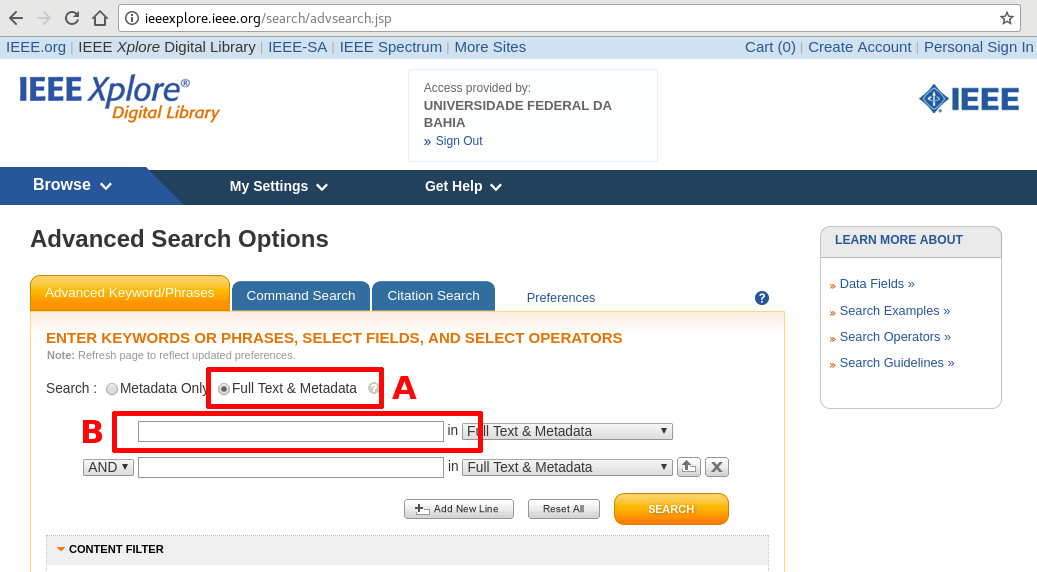
\includegraphics[scale=0.4]{imagens/advanced-search-ieee.png}}
  \caption{Captura de tela da busca avançada da base IEEE com destaque para a (A) opção de busca completa e para o (B) campo de entrada da string de busca.}
  \label{advanced-search-ieee}
\end{figure}

A busca avançada na base ACM (Figura \ref{advanced-search-acm}) não necessita
marcar nenhum campo adicional além do próprio campo texto onde deve-se entrar
com a string de busca de cada projeto.

\begin{figure}[h]
  \center
  \frame{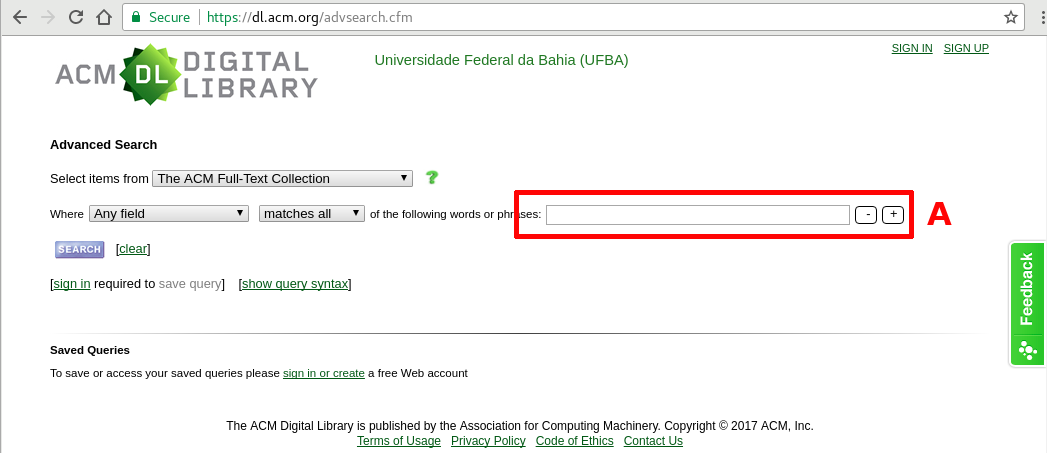
\includegraphics[scale=0.4]{imagens/advanced-search-acm.png}}
  \caption{Captura de tela da busca avançada da base ACM com destaque para o (A) campo de entrada da string de busca.}
  \label{advanced-search-acm}
\end{figure}

Para cada projeto de software são construídas duas strings, uma para busca na
base da ACM, outra para busca na base IEEE, os resultados da busca de cada
string são armazenados localmente em arquivos no formato BibTeX, ambas as bases
exportam os resultados neste formato.

As strings de busca são elaboradas a partir dos dados coletados no estudo
anterior, como, nome do projeto, descrição, nome do autor da publicação
original, entre outros dados. A elaboração das strings é realizada num processo
incremental e iterativo, iniciando por uma busca utilizando apenas o nome do
projeto, avaliando os resultados, inspecionando o título de cada resultado,
refinando a string através de outras características do projeto quando os
resultados trazem muitos estudos sem relação com o projeto de software.

%buscamos inicialmente usando apenas o nome do software, analisamos o número total
%de resultados e os títulos destes resultados, quando o número de resultados for
%muito grande, acima de XXX, e os títulos não aparentavam ser estudos com relação
%aos projetos, incluímos mais características, como por exemplo, parte da descrição
%do software, ou parte da URL, autores, etc.

%% Cuidado que ACM cita IEEE.
Os resultados trazidos pela string final são armazenados localmente em formato
BibTeX, são dois arquivos para cada projeto de software, um contendo os
resultados da busca na base ACM -- \texttt{acm.bib} -- e outro contendo os
resultados da base IEEE -- \texttt{ieee.bib}.

%e pdf,
%estes resultados devem incluir ao menos os artigos selecionados
%no estudo anterior onde os projetos foram encontrados, já que tais artigos são
%o caso mínimo de resultado desejado nesta fase de busca. 

O resultado final da busca de todos os projetos, armazenados nos arquivos
\texttt{acm.bib} e \texttt{ieee.bib}, são agregados sem duplicação de resultado
num arquivo único ainda em formato BibTeX localizado em
\texttt{documents/references.bib},
este arquivo contém os metadados de todos os artigos encontrados pelas strings
de busca de cada projeto nas bases ACM e IEEE.

Este arquivo além de eliminar as duplicidades de resultados recebe também para
cada item uma identificação única, esta identificação será utilizada nas etapas
seguintes da revisão de literatura para fazer relacionar os projeto com os
artigos através das menções.

%de cada projeto, sem duplicidade, cada artigo receberá um ID único, este ID
%será utilizado nas etapas seguintes.

%, e um com um merge destes dois mantendo resultados únicos sem
%duplicidade.

%Para cada software, os resultados foram agrupados
%num arquivo único, sem duplicidade entre os resultados trazidos por cada base
%bibliográfica. O arquivo de metadados de cada software contém informações sobre
%o artigo, autores, ano de publicação, conferência, jornal, etc. Os artigos
%também foram armazenados localmente, no formato pdf para serem analisados na
%triagem.

\subsection{Passo 2: Triagem}

% leitura dos pdf > apenas os papers relevantes que mencionam o nome do software

Neste passo selecionamos os artigos relevantes para cada projeto, identificando
nos resultados da busca avançada de cada string, através de inspeção manual do
artigo, se ele faz menção ao projeto realmente. A primeira ação neste passo é
fazer o download de cada artigo em formato pdf presente no arquivo
\texttt{documents/references.bib} para inspeção manual.

Os artigos encontrados no passo anterior serão inspecionados manualmente em
busca de confirmar se fazem referência de fato aos projetos de software,
os dados gerados neste passo são armazenados no arquivo \texttt{software.yml} de cada projeto,
fazendo referência sempre ao ID do artigo definido no passo anterior.

A inspeção tem como objetivo selecionar os artigos relevantes para este estudo,
mantendo apenas aqueles com menção ao nome do software, seja a menção em
formato de citação formal ou informal, cada resultado é armazenado no yml
através do campo \texttt{really\_refers\_to\_software}, recebendo os valores
\texttt{yes} ou \texttt{no}, ser atualizado com o resultado da triagem,
indicando se faz referência ao nome do projeto ou não.

%de cada artigo é realizada com o auxílio da funcionalidade de busca
%do leitor de pdf utilizado neste estudo\footnote{Utilizamos software Evince v3.22.1}
%utilizado para leitura dos artigos, com o auxílio da busca encontramos cada
%ocorrência ao nome do software tomando nota a confirmação sobre a menção
%encontrada.

%Esta informação foi armazenada no próprio arquivo BibTeX num campo adicional
%aos demais campos dos metadados do artigo; ao final, temos os metadados do
%artigo como, título, autores, ano de publicação, etc, e também uma indicação se
%o artigo cita realmente o software.

\subsection{Passo 3: Keywording}

% papers relevantes > esquema de tipos de menção

Nesta fase da revisão de literatura criamos o esquema de codificação para
classificação das menções, o esquema é criado a partir da identificação do
contexto em que os projetos são mencionados em cada artigo, para cada menção
toma-se nota sobre como o software é mencionado naquele artigo.

As notas são comentários livres resumindo as menções encontradas no artigo
sobre um determinado software, um artigo científico pode mencionar um software
diversas vezes, de diversas formas, desde uma simples menção nos trabalhos
relacionados até uma grande contribuição ao software, este dado é coletado no
campo texto livre \texttt{review} no yml de cada software.

O conjunto final de todas as notas são agrupadas e analisadas individualmente
com o objetivo de criar a partir dessas notas um conjunto mínimo de códigos
para classificação de menções a software acadêmico. Este esquema deve ser construído
como uma escala de pesos, onde o último tipo de menção inclui implicitamente os
tipos de menor peso.

%Esta leitura irá gerar
%uma escala de tipos de menção ao software. Cada artigo assume, em relação ao
%software, um valor nesta escala de tipos de menção.

%Foi lido em busca de encontrar menções ao nome do software, em qual contexto o
%software é mencionado e de que forma é mencionado, resume cada tipo de menção com explicação dos casos em
%que se enquadram, o método utilizado para.

\subsection{Passo 4: Extração}

A partir do esquema para classificação das menções extraímos para cada artigo
qual o tipo de menção ele faz ao software, quando o artigo menciona o software
diversas vezes adotamos o tipo de menção com maior peso, indicando que os pesos
menores estão incluídos.

%A partir da classificação , Tabela \ref{esquema-de-mencao}, extraímos de cada
%artigo mencionando os projetos de acordo com o esquema de codificação criado no

A extração desses dados devem ser armazenadas no próprio arquivo yml, sendo
atualizado com a inclusão de um novo campo indicando o tipo de menção do artigo
ao software.

Ao final da revisão de literatura teremos para cada projeto de software um
conjunto de artigos com menções classificadas por tipo e contexto, estando
incluído nestes conjuntos ao menos os próprios artigos que deram origem ao
conjunto de projetos utilizados como objeto de estudo neste trabalho.

%menções a eles nas bases do ACM e IEEE, temos o tipo de cada menção, se
%contribuiu com o projeto, se foi avaliado, ou apenas citado como referência, os
%artigos selecionados no estudo anterior que deram origem ao conjunto de
%projetos de software estão incluídos nestes resultados.

% }}}

\section{Preparação} \label{estudo2:preparacao} % {{{

\subsection{Passo 1: Busca}

Criamos as strings de busca. A Tabela ... apresenta a
string de busca de alguns projetos de software na base ACM e na base IEEE.
Um documento CSV com todas as strings de busca pode ser encontrado no
repositório\footnote{\url{https://github.com/joenio/dissertacao-ufba-2016}}
desta dissertaçao no arquivo \texttt{documents/search-strings.csv}.

As strings foram registradas no arquivo \texttt{software.yml} de cada software,
foram criados também campos para registrar o número de resultados da busca
e a data em que a busca foi realizada registrada no formato UTC.

Segue abaixo um exemplo do trecho do arquivo \texttt{software.yml} com os campos
para armazenar os dados da busca, Figura \ref{software-yml-exemplo}.

\begin{figure}[h]
  \begin{verbatim}
  search:
    acm:
      string: content.ftsec:(+AccessAnalysis +Tool +Java +Modifiers)
      searched_at: Sun Aug  6 21:45:40 UTC 2017
      results: 5
    ieee:
      string: (AccessAnalysis)
      searched_at: Sun Jul 30 15:46:57 UTC 2017
      results: 3
  \end{verbatim}
  \caption{Trecho do arquivo software.yml do projeto AccessAnalysis.}
  \label{software-yml-exemplo}
\end{figure}


\subsection{Passo 2: Triagem}

...

\subsection{Passo 3: Keywording}

...

\subsection{Passo 4: Extração}

...

Implementamos scripts para análise dos dados. Os dados armazenados em arquivos
YAML e BibTeX são carregados em estruturas em memória através de um script
escrito em linguagem Perl e repassados para templates processados para exibir
os dados neste texto, em arquivos TeX, CSV, etc. A Figura \ref{estudo2-fluxograma}
apresenta o fluxo de coleta, análise e transformação dos dados.

\begin{figure}[h]
  \center
  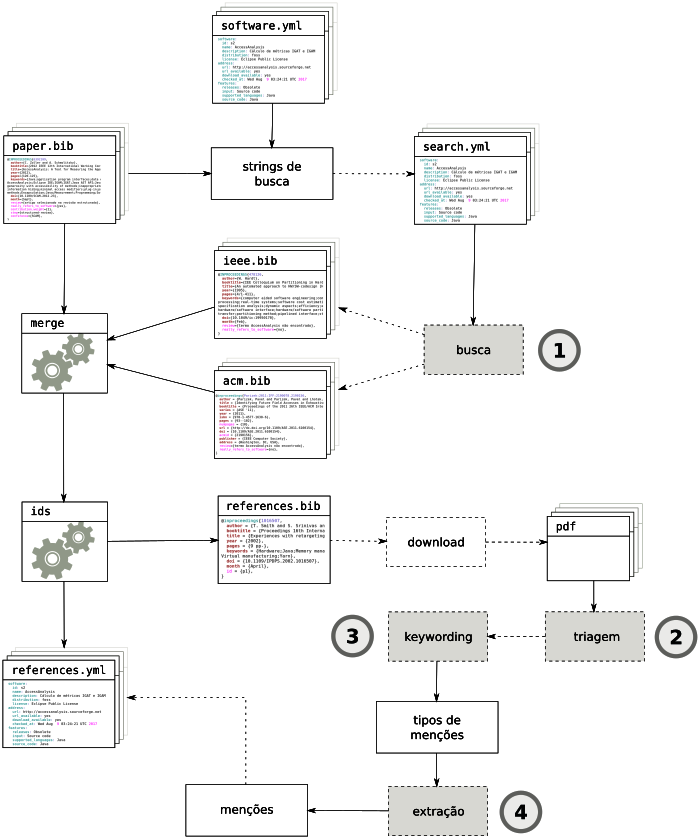
\includegraphics[scale=0.4]{imagens/estudo2-fluxograma.png}
  \caption{Fluxo de coleta, análise e transformação dos dados.}
  \label{estudo2-fluxograma}
\end{figure}

Implementamos os scripts \texttt{bin/summarize-dataset}, \texttt{bin/query},
\texttt{bin/clean}, \texttt{bin/ids} e \texttt{bin/render-template} indicados
no fluxograma da Figura \ref{estudo2-fluxograma} utilizando a linguagem de
programação Perl\footnote{\url{http://perl.org}} com o auxílio dos seguintes
módulos CPAN: Modern::Perl\footnote{\url{http://metacpan.org/pod/Modern::Perl}},
YAML\footnote{\url{http://metacpan.org/pod/YAML}},
Mojo::Template\footnote{\url{http://metacpan.org/pod/Mojo::Template}},
Text::BibTeX\footnote{\url{http://metacpan.org/pod/Text::BibTeX}} e
List::Util\footnote{\url{http://metacpan.org/pod/List::Util}}. A maior parte da
lógica de implementação destes scripts foram movidas para o arquivo
\texttt{lib/Dissertacao.pm} com objetivo de reduzir repetição de código e
aumentar o reuso.

Definimos uma identificação única para cada um dos 60 projetos de software
utilizando o próprio arquivo \texttt{software.yml} através do campo
\texttt{id:} seguindo o padrão \texttt{s + número}, exemplo, \texttt{s1},
\texttt{s2}, \texttt{s3}, \texttt{s4}, ..., \texttt{s60}, cada projeto de software
recebeu um id.

Definimos um novo campo neste mesmo arquivo para coleta das menções, fazendo
referência ao ID do artigo mencionando o software, com os campos ... cada artigo
encontrado na revisão de literatura também receberá um ID, desta forma será possível
relacionar projetos e artigos através das menções.

% }}}

\section{Coleta de dados}

Seguindo o planejamento e preparação descritos nas seções
\ref{estudo2:planejamento} e \ref{estudo2:preparacao} iniciamos a coleta dos
dados através da revisão de literatura nas bases ACM e IEEE.

% dados do estudo1
\newcommand{\SoftwareCount}{60}
\newcommand{\SoftwareUrlNotAvailableCount}{15}
\newcommand{\SoftwareUrlAvailableCount}{45}
\newcommand{\SoftwareDownloadNotAvailableCount}{24}
\newcommand{\SoftwareDownloadAvailableCount}{36}
% dados do estudo2
\newcommand{\SearchACMCount}{438}
\newcommand{\SearchIEEECount}{459}
\newcommand{\SearchCount}{897}
\newcommand{\SearchUniqueCount}{806}
\newcommand{\ScreeningCount}{429}
\newcommand{\ScreeningUniqueCount}{416}
\newcommand{\CiteCount}{199}
\newcommand{\UseCount}{124}
\newcommand{\ContributeCount}{106}
\newcommand{\SearchUniqueMean}{13.4}
\newcommand{\ScreeningMean}{7.2}
\newcommand{\ScreeningUniqueMean}{6.9}
\newcommand{\MentionsStudyUm}{60}
\newcommand{\MentionsStudyDois}{47}
\newcommand{\SoftwareNotMentionedCount}{13}
\newcommand{\ContributeStudyDoisCount}{43}
\newcommand{\ContributeStudyDoisSoftware}{17}
% dados do estudo3
\newcommand{\ReleasesCount}{303}
\newcommand{\ReleasesAvailableCount}{211}
\newcommand{\ReleasesMetricsCount}{206}
\newcommand{\ProjectsWithReleasesCount}{35}
\newcommand{\ProjectsAnalizedCount}{24}
\newcommand{\ReleasesYearFirst}{2001}
\newcommand{\ReleasesYearLast}{2017}


\subsection{Passo 1: Busca}

Uma string de busca foi definida para cada software acadêmico selecionado.
Além do nome do software pesquisado, as strings de busca incluíram outras
características do software sempre que necessário.

Encontramos um total de \SearchCount \ resultados usando as strings de busca
para cada projeto nas bases ACM e IEEE, deste total \SearchACMCount \ resultados
foram encontrados na base ACM e \SearchIEEECount \ foram encontrados
no IEEE. Dentre o resultado total, \SearchUniqueCount \ são únicos.

Alguns artigos fazem menção a mais de 1 projeto, fizemos o download de cada
artigo e armazenamos os metadados em formato BibTeX nos arquivos \texttt{acm.bib}
e \texttt{ieee.bib} para cada projeto de software.

\subsection{Passo 2: Triagem}

Inspecionamos cada um dos \SearchUniqueCount \ artigos em busca de menções ao
nome do projeto de software associado com a busca que retornou estes artigos,
nesta busca utilizamos como critério qualquer ocorrencia ao nome do projeto de
software mas que seja realmente referente ao software em sí, alguns projetos de
software do nosso conjunto possui nomes comuns que foram encontrados nos
artigos mas não faziam referencia ao software, em alguns casos os nomes
apareciam em fórmulas matemáticas ou como parte de um outra palavra.

Ao final selecionamos para cada projeto um conjunto de artigos que de fato
mencionam o software, ainda sem caracterizar o tipo de menção, apenas se
realmente menciona, ao total selecionamos \ScreeningCount \ menções.
Este total de menções foram encontrados ao meio a \ScreeningUniqueCount \ artigos.

Uma tabela no formato CSV com todas as referências pode ser encontrada no repositório
desta dissertação no arquivo \texttt{documents/references.csv}, neste arquivo todos
os artigos e todos os projetos são representados e a relação entre eles é marcada com
um \texttt{x} sempre que houver menção de um artigo para um software.

Merge único de todos os arquivos BibTeX, incluindo o arquivo \texttt{paper.bib} de
cada projeto gerado no estudo anterior apresentado no Capítulo \ref{estudo1}, um
arquivo \texttt{documents/references.bib} foi criado contendo todas as referências
a todos os projetos, referências únicas.

Na sequencia adicionamos o \texttt{id} a cada artigo do
\texttt{documents/references.bib}, este arquivo tem os metadados dos artigos
encontrados fazendo menção aos projetos, eles receberam ids, estes ids serão
utilizados para relacionar o projeto ao artigo.

Os scripts \texttt{bin/query}, \texttt{bin/clean}, \texttt{bin/ids} foram
utilizados para gerar o \texttt{documents/references.bib} a partir dos arquivos
\texttt{acm.bib}, \texttt{ieee.bib} e \texttt{paper.bib} de cada projeto.

334 artigos fazem menção aos 60 projetos.
350 não faz menção aos projetos.

\subsection{Passo 3: Keywording}

A avaliação das \ScreeningCount \ menções gerou uma escala de tipos de menção
ao software, detalhado na Tabela \ref{esquema-de-mencao}, com três valores
distintos, onde o último tipo de menção com maior valor inclui todos os demais.
Um tipo de menção com maior peso inclui implicitamente o tipo de menção de
menor peso, e assim sucessivamente.

\begin{table}[h]
\caption{Esquema para classificação de menções aos projetos software acadêmico.}
\centering
\begin{tabular}{ l p{10cm} }
  \hline
  Tipo de menção           & Explicação \\
  \hline
  Cita      & Apenas cita o software ou é o mesmo artigo onde o software selecionado; É um artigo com ``mesmo'' conteúdo publicado na ``mesma'' época; O artigo apenas descreve o software; Menciona o software numa tabela com outros, classifica; Menciona o software como exemplo; Menciona o software como trabalho relacionado; Menciona o software em trabalhos futuros. \\
  Usa       & Avalia ou caracteriza o software; Usa para coleta ou análise de dados; Usa como objeto de estudo; Usa o software como parte de uma solução, implementação, etc; Cria um software derivado mas não disponibiliza as contribuições. \\
  Contribui & Cria; Contribuição inicial criando o projeto; Faz uma grande contribuição; Refatora todo o software; Abre o código de um software que antes era de código fechado; Contribuição pequena ou moderada; Extende o software; Integra o software a outros sistemas, formatos de entrada/saída, APIs, etc (seja implementando suporte no software ou do outro lado); Refatora parte do software; Implementa parte do software em outro projeto e compara resultados. \\
  \hline
\end{tabular}
\label{esquema-de-mencao}
\end{table}

A definição deste esquema foi feito através de anotações sobre onde
e como o projeto de software é mencionado em cada artigo, anotamos no campo
\texttt{review:} um comentário textual livre resumindo de que forma o projeto
é mencionado, caso várias menções seja encontrado num mesmo artigo para um dado
projeto de software é feito um resumo total.

Esta anotação foi feita no arquivo \texttt{software.yml} de cada projeto, nele
foi adicionado um novo registro para cada artigo que faz menção e notas sobre a
menção foi adicionada. É importante lembrar que um mesmo artigo pode mencionar
mais de um software.

%também o tipo de menção que é feita ao software: se apenas cita como exemplo,
%se contribui com novos algoritmos e técnicas, se avalia, ou apenas descreve o
%software comparando-o com outro software.

\subsection{Passo 4: Extração}

Coletamos as informações relacionadas a cada menção encontrada, cada um dos
\ScreeningUniqueCount \ artigos encontrados mencionando os projetos, coletamos
como o projeto é mencionado, encontramos \ScreeningCount \ menções aos
projetos neste conjunto de artigos.

A partir do esquema para caracterização das menções adicionamos para
cada projeto de software os campos \texttt{really\_refers\_to\_software:}
com o valor \texttt{yes}, o campo \texttt{contribution\_weight:} assumindo
os valores: 0.1 (cita), 0.25 (usa), 0.5 (contribui), 1 (contribui).

Os dados coletados na revisão de literatura durante os quatro passos são
apresentados em resumo na Tabela ... indicando o
número de resultados encontrados para cada projeto de software.

%
\begin{longtable}{ l c c c c c }
\caption{Resumo dos resultados encontrados na revisão de literatura.}
\label{literature-review-table} \\
  \hline
  \hhline{ l c c c c c |}
  \endfirsthead
  \hhline{ l c c c c c |}
  \hline
   \multirow{2}{*}{\textbf{Nome do software}} & \multicolumn{5}{c}{{\bf Menções}} \\
   & \textbf{Cita} & \textbf{Usa} & \textbf{Contribui} & \textbf{Cria} & \textbf{Total} \\
  \hline
  \hhline{ l c c c c c |}
  \endhead
  \hhline{------}
  \multicolumn{6}{c}{continua na próxima página} \\
  \hhline{------} \endfoot
  \hhline{------} \endlastfoot
   \multirow{2}{*}{\textbf{Nome do software}} & \multicolumn{5}{c}{{\bf Menções}} \\
   & \textbf{Cita} & \textbf{Usa} & \textbf{Contribui} & \textbf{Cria} & \textbf{Total} \\
  \hline
   2LS & 0 & 0 & 0 & 1 & 1 \\
   AccessAnalysis & 1 & 0 & 0 & 1 & 2 \\
   APIExample & 3 & 0 & 0 & 1 & 4 \\
   BEG & 4 & 3 & 1 & 1 & 9 \\
   ccJava & 2 & 0 & 2 & 1 & 5 \\
   CIVL & 4 & 0 & 0 & 1 & 5 \\
   CodeBoost & 9 & 0 & 0 & 1 & 10 \\
   CSL & 3 & 1 & 1 & 1 & 6 \\
   CPA+ & 0 & 0 & 4 & 1 & 5 \\
   CSeq & 1 & 2 & 1 & 1 & 5 \\
   DDVerify & 2 & 0 & 0 & 1 & 3 \\
   Derailer & 1 & 0 & 0 & 1 & 2 \\
   Diagnosys & 0 & 0 & 0 & 1 & 1 \\
   DOMPLETION & 1 & 0 & 0 & 1 & 2 \\
   DRC & 4 & 0 & 0 & 1 & 5 \\
   e-munity & 0 & 0 & 0 & 1 & 1 \\
   EJB & 1 & 1 & 0 & 2 & 4 \\
   Error Prone & 0 & 1 & 0 & 1 & 2 \\
   ESBMC & 14 & 18 & 7 & 1 & 40 \\
   ETXL & 0 & 0 & 0 & 1 & 1 \\
   FaultBuster & 0 & 0 & 0 & 1 & 1 \\
   Flowgen & 2 & 0 & 0 & 1 & 3 \\
   GRT & 3 & 2 & 1 & 2 & 8 \\
   GUIZMO & 0 & 0 & 0 & 1 & 1 \\
   GumTree & 5 & 10 & 2 & 1 & 18 \\
   HUSACCT & 3 & 2 & 0 & 2 & 7 \\
   Indus & 0 & 2 & 0 & 1 & 3 \\
   JastAdd & 22 & 14 & 2 & 1 & 39 \\
   JFlow & 5 & 1 & 0 & 1 & 7 \\
   JstereoCode & 2 & 5 & 0 & 1 & 8 \\
   Jtop & 0 & 1 & 0 & 1 & 2 \\
   Bogor/Kiasan & 8 & 0 & 5 & 1 & 14 \\
   Loopfrog & 2 & 2 & 0 & 1 & 5 \\
   Lotrack & 1 & 0 & 0 & 1 & 2 \\
   MPAnalyzer & 0 & 0 & 0 & 1 & 1 \\
   MSP & 1 & 0 & 0 & 1 & 2 \\
   mygcc & 3 & 1 & 1 & 2 & 7 \\
   PARSEWeb & 17 & 0 & 0 & 1 & 18 \\
   PAT & 1 & 0 & 0 & 1 & 2 \\
   PHP AiR & 1 & 5 & 2 & 1 & 9 \\
   protopurity & 0 & 0 & 0 & 1 & 1 \\
   Pseudogen & 0 & 0 & 0 & 1 & 1 \\
   PtYasm & 0 & 0 & 0 & 2 & 2 \\
   PuMoC & 1 & 0 & 0 & 1 & 2 \\
   PYTHIA & 0 & 0 & 1 & 1 & 2 \\
   ReAssert & 9 & 3 & 0 & 1 & 13 \\
   Rêve & 0 & 0 & 0 & 1 & 1 \\
   RRFinder & 1 & 0 & 0 & 1 & 2 \\
   Sapid/XML & 1 & 2 & 1 & 1 & 5 \\
   Sonar Qube Plug-in & 0 & 0 & 0 & 1 & 1 \\
   SPARTA & 1 & 2 & 0 & 1 & 4 \\
   srcML & 14 & 23 & 2 & 1 & 40 \\
   SWAT & 1 & 2 & 0 & 1 & 4 \\
   TACLE & 1 & 1 & 0 & 1 & 3 \\
   TEBA & 0 & 0 & 0 & 1 & 1 \\
   TestEra & 15 & 5 & 0 & 1 & 21 \\
   Vdiff & 4 & 0 & 0 & 1 & 5 \\
   WALA & 5 & 5 & 0 & 1 & 11 \\
   Wrangler & 16 & 10 & 6 & 1 & 33 \\
   XOgastan & 4 & 0 & 0 & 1 & 5 \\
  \hline
  {\bf Total} & 199 & 124 & 39 & 65 & 427 \\
\end{longtable}


A Figura \ref{mentions-timeline} apresenta uma visualização da linha do tempo
de cada software em relação a menções encontradas nas bases ACM e IEEE através
da revisão de literatura.

\begin{figure}[h]
  \center
  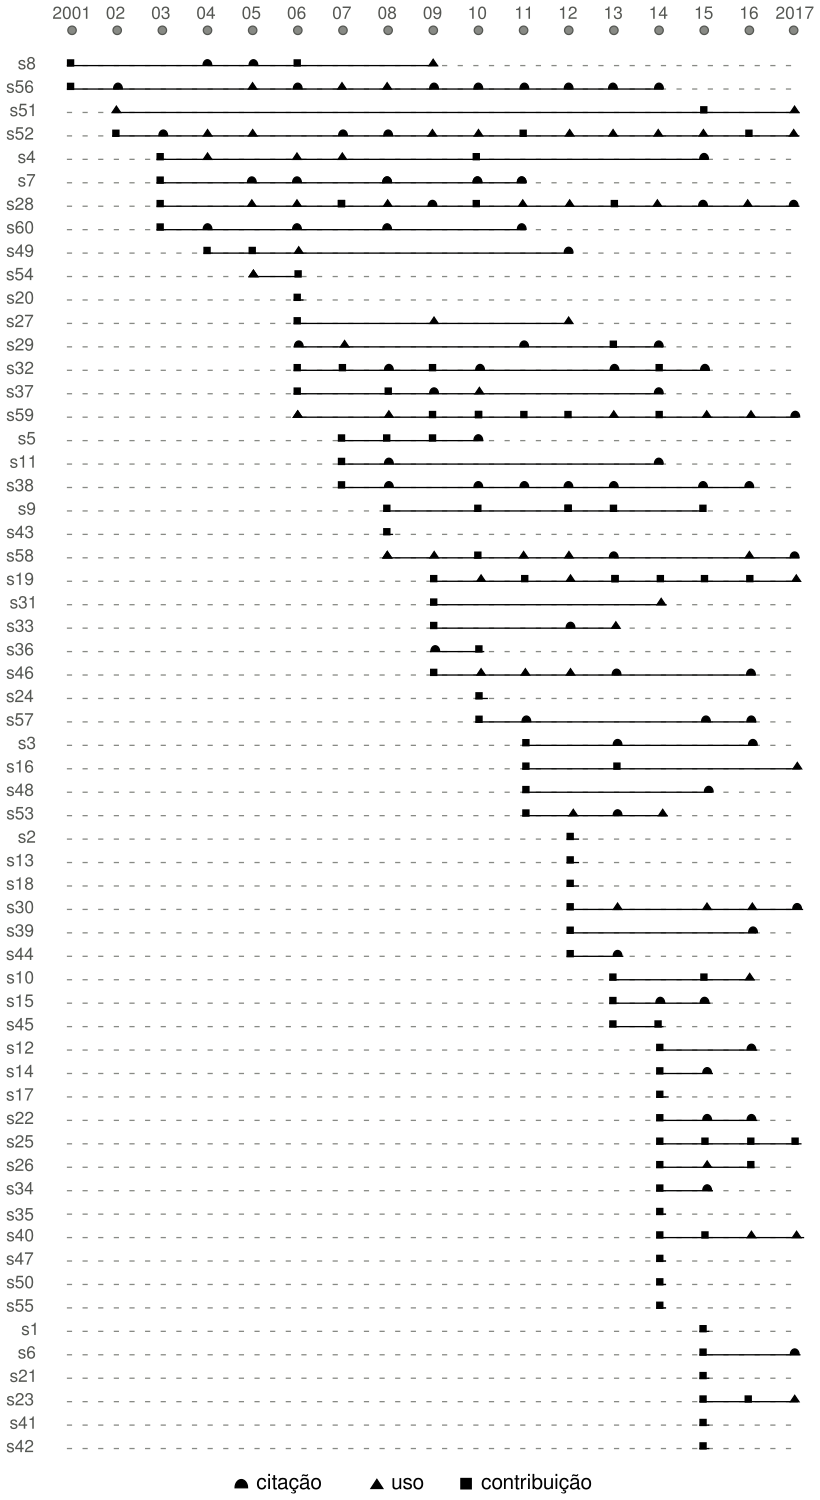
\includegraphics[scale=0.7]{imagens/mentions-timeline.png}
  \caption{Linha do tempo de menções (uso e contribuição) aos projetos nas bases ACM e IEEE.}
  \label{mentions-timeline}
\end{figure}

\section{Análise dos Dados} % Raw results from the analysis

Dados de 60 projetos de software acadêmico de análise estática desenvolvidos e
publicados na literatura acadêmica de engenharia de software, informações sobre
diversas formas de menção ao nome destes projetos na literatura acadêmica.
%o número de autores mencionando o software ao longo do tempo.

\subsection{Passo 1: Busca}

...

\subsection{Passo 2: Triagem}

...

\subsection{Passo 3: Keywording}

...

\subsection{Passo 4: Extração}

...

\section{Interpretação dos Resultados} % Hypothesis rejection

... a Tabela \ref{visibility-table} ...

%

\begin{longtable}{ l *{17}{c} }
\caption{Número de menções por ano (de 2001 até 2017).}
\label{authorship-table} \\
  \hline
  \hhline{ l *{17}{c} |}
  \endfirsthead
  \hhline{ l *{17}{c} |}
  \hline
  \textbf{Projeto} & 1 & 2 & 3 & 4 & 5 & 6 & 7 & 8 & 9 & 10 & 11 & 12 & 13 & 14 & 15 & 16 & 17 \\
  \hline
  \hhline{ l *{17}{c} |}
  \endhead
  \hhline{------------------}
  \multicolumn{17}{c}{continua na próxima página} \\
  \hhline{------------------} \endfoot
  \hhline{------------------} \endlastfoot
  \textbf{Projeto} & 1 & 2 & 3 & 4 & 5 & 6 & 7 & 8 & 9 & 10 & 11 & 12 & 13 & 14 & 15 & 16 & 17 \\
  \hline
    2LS & - & - & - & - & - & - & - & - & - & - & - & - & - & - & HASH(0x55bf7861a9e8) & - & - \\
    AccessAnalysis & - & - & - & - & - & - & - & - & - & - & - & HASH(0x55bf785f3850) & - & - & - & - & - \\
    APIExample & - & - & - & - & - & - & - & - & - & - & HASH(0x55bf785f7f60) & - & HASH(0x55bf785f8140) & - & - & HASH(0x55bf784c87c0) & - \\
    BEG & - & - & HASH(0x55bf78604500) & HASH(0x55bf78604698) & - & HASH(0x55bf784c58d0) & HASH(0x55bf786047a0) & - & - & HASH(0x55bf78604668) & - & - & - & - & HASH(0x55bf784c5960) & - & - \\
    ccJava & - & - & - & - & - & - & HASH(0x55bf78618b28) & HASH(0x55bf78619b18) & HASH(0x55bf784cc760) & HASH(0x55bf78619c68) & - & - & - & - & - & - & - \\
    CIVL & - & - & - & - & - & - & - & - & - & - & - & - & - & - & HASH(0x55bf7858a380) & - & HASH(0x55bf7858a578) \\
    CodeBoost & - & - & HASH(0x55bf78606f70) & - & HASH(0x55bf78607108) & HASH(0x55bf784c5e40) & - & HASH(0x55bf78607258) & HASH(0x55bf786072b8) & HASH(0x55bf78607318) & HASH(0x55bf78607378) & HASH(0x55bf786073d8) & HASH(0x55bf78607438) & - & HASH(0x55bf78607498) & - & - \\
    CSL & HASH(0x55bf786279e8) & - & - & HASH(0x55bf78627bb0) & HASH(0x55bf784dd4a8) & HASH(0x55bf78627cb8) & - & - & HASH(0x55bf78627d18) & - & - & - & - & - & - & - & - \\
    CPA+ & - & - & - & - & - & - & - & HASH(0x55bf785892a0) & - & HASH(0x55bf785894c8) & - & HASH(0x55bf784bc0b0) & HASH(0x55bf785895d0) & - & HASH(0x55bf78589630) & - & - \\
    CSeq & - & - & - & - & - & - & - & - & - & - & - & - & HASH(0x55bf7861c668) & - & HASH(0x55bf7861c8b0) & HASH(0x55bf784d9470) & - \\
    DDVerify & - & - & - & - & - & - & HASH(0x55bf785f8908) & HASH(0x55bf785f9910) & - & - & - & - & - & HASH(0x55bf784c8a30) & - & - & - \\
    Derailer & - & - & - & - & - & - & - & - & - & - & - & - & - & HASH(0x55bf7857d2f8) & - & HASH(0x55bf7857d508) & - \\
    Diagnosys & - & - & - & - & - & - & - & - & - & - & - & HASH(0x55bf78622ac0) & - & - & - & - & - \\
    DOMPLETION & - & - & - & - & - & - & - & - & - & - & - & - & - & HASH(0x55bf785f11d0) & HASH(0x55bf785f13b0) & - & - \\
    DRC & - & - & - & - & - & - & - & - & - & - & - & - & HASH(0x55bf78591368) & HASH(0x55bf78591530) & HASH(0x55bf784ba840) & - & - \\
    e-munity & - & - & - & - & - & - & - & - & - & - & - & - & - & HASH(0x55bf7862cfd8) & - & - & - \\
    EJB & - & - & - & - & - & - & - & - & - & - & HASH(0x55bf7860f870) & - & HASH(0x55bf7860fa08) & - & - & - & HASH(0x55bf784d1538) \\
    Error Prone & - & - & - & - & - & - & - & - & - & - & - & HASH(0x55bf78602428) & - & - & HASH(0x55bf78602680) & - & - \\
    ESBMC & - & - & - & - & - & - & - & - & HASH(0x55bf785e3e30) & HASH(0x55bf785e4028) & HASH(0x55bf784c17c8) & HASH(0x55bf785e4130) & HASH(0x55bf785e3ff8) & HASH(0x55bf785e4238) & HASH(0x55bf784c1858) & HASH(0x55bf785e3e90) & HASH(0x55bf784c18d0) \\
    ETXL & - & - & - & - & - & HASH(0x55bf785f53e8) & - & - & - & - & - & - & - & - & - & - & - \\
    FaultBuster & - & - & - & - & - & - & - & - & - & - & - & - & - & - & HASH(0x55bf78609230) & - & - \\
    Flowgen & - & - & - & - & - & - & - & - & - & - & - & - & - & HASH(0x55bf7861d0f0) & HASH(0x55bf7861d288) & HASH(0x55bf784d9710) & - \\
    GRT & - & - & - & - & - & - & - & - & - & - & - & - & - & HASH(0x55bf78625708) & HASH(0x55bf78625630) & HASH(0x55bf784dcf80) & HASH(0x55bf78625780) \\
    GUIZMO & - & - & - & - & - & - & - & - & - & HASH(0x55bf7862b2f0) & - & - & - & - & - & - & - \\
    GumTree & - & - & - & - & - & - & - & - & - & - & - & - & - & HASH(0x55bf785ff928) & HASH(0x55bf785ffb50) & HASH(0x55bf784cb058) & HASH(0x55bf785ff9b8) \\
    HUSACCT & - & - & - & - & - & - & - & - & - & - & - & - & - & HASH(0x55bf7857eff8) & HASH(0x55bf7857f190) & HASH(0x55bf7847a220) & - \\
    Indus & - & - & - & - & - & HASH(0x55bf78635c48) & - & - & HASH(0x55bf78635db0) & - & - & HASH(0x55bf784d8740) & - & - & - & - & - \\
    JastAdd & - & - & HASH(0x55bf78616598) & - & HASH(0x55bf78616748) & HASH(0x55bf784cc0e8) & HASH(0x55bf786165f8) & HASH(0x55bf784cc148) & HASH(0x55bf784cc0d0) & HASH(0x55bf78616718) & HASH(0x55bf78616b80) & HASH(0x55bf784cc250) & HASH(0x55bf784cc2e0) & HASH(0x55bf784cc328) & HASH(0x55bf784cc1d8) & HASH(0x55bf784cc3d0) & HASH(0x55bf78617dc0) \\
    JFlow & - & - & - & - & - & HASH(0x55bf78590558) & HASH(0x55bf78590768) & - & - & - & HASH(0x55bf784ba510) & - & HASH(0x55bf78590870) & HASH(0x55bf785908d0) & - & - & - \\
    JstereoCode & - & - & - & - & - & - & - & - & - & - & - & HASH(0x55bf78600d80) & HASH(0x55bf78600b28) & - & HASH(0x55bf784cb478) & HASH(0x55bf78600eb8) & HASH(0x55bf78601098) \\
    Jtop & - & - & - & - & - & - & - & - & HASH(0x55bf785f4e60) & - & - & - & - & HASH(0x55bf785f50d0) & - & - & - \\
    Bogor/Kiasan & - & - & - & - & - & HASH(0x55bf78620978) & HASH(0x55bf78620af8) & HASH(0x55bf784d9bd8) & HASH(0x55bf784d9c20) & HASH(0x55bf78620cf0) & - & - & HASH(0x55bf786209c0) & HASH(0x55bf78620df8) & HASH(0x55bf78620e58) & - & - \\
    Loopfrog & - & - & - & - & - & - & - & - & HASH(0x55bf7862ad98) & - & - & HASH(0x55bf7862af30) & HASH(0x55bf784dd9b8) & - & - & - & - \\
    Lotrack & - & - & - & - & - & - & - & - & - & - & - & - & - & HASH(0x55bf785f3160) & HASH(0x55bf785f3328) & - & - \\
    MPAnalyzer & - & - & - & - & - & - & - & - & - & - & - & - & - & HASH(0x55bf784dd058) & - & - & - \\
    MSP & - & - & - & - & - & - & - & - & HASH(0x55bf7858bd30) & HASH(0x55bf7858bee0) & - & - & - & - & - & - & - \\
    mygcc & - & - & - & - & - & HASH(0x55bf785f7258) & - & HASH(0x55bf785f73d8) & HASH(0x55bf784c84a8) & HASH(0x55bf785f74e0) & - & - & - & HASH(0x55bf785f7540) & - & - & - \\
    PARSEWeb & - & - & - & - & - & - & HASH(0x55bf7860de80) & HASH(0x55bf7860e078) & - & HASH(0x55bf784d11c0) & HASH(0x55bf7860dee0) & HASH(0x55bf7860e228) & HASH(0x55bf7860e288) & - & HASH(0x55bf7860e2e8) & HASH(0x55bf7860e348) & - \\
    PAT & - & - & - & - & - & - & - & - & - & - & - & HASH(0x55bf78623530) & - & - & - & HASH(0x55bf78623698) & HASH(0x55bf784dcba8) \\
    PHP AiR & - & - & - & - & - & - & - & - & - & - & - & - & - & HASH(0x55bf78633bc0) & HASH(0x55bf78633d40) & HASH(0x55bf784d8248) & HASH(0x55bf784d8290) \\
    protopurity & - & - & - & - & - & - & - & - & - & - & - & - & - & - & HASH(0x55bf785e79a8) & - & - \\
    Pseudogen & - & - & - & - & - & - & - & - & - & - & - & - & - & - & HASH(0x55bf78631c38) & - & - \\
    PtYasm & - & - & - & - & - & - & - & HASH(0x55bf785e4b08) & - & - & - & - & - & - & - & - & - \\
    PuMoC & - & - & - & - & - & - & - & - & - & - & - & HASH(0x55bf78580838) & HASH(0x55bf78580a30) & - & - & - & - \\
    PYTHIA & - & - & - & - & - & - & - & - & - & - & - & - & HASH(0x55bf785f9eb0) & HASH(0x55bf785fa0a8) & - & - & - \\
    ReAssert & - & - & - & - & - & - & - & - & HASH(0x55bf785f0740) & HASH(0x55bf785f0938) & HASH(0x55bf784bec70) & HASH(0x55bf785f0a40) & HASH(0x55bf785f0908) & - & - & HASH(0x55bf784bed00) & - \\
    Rêve & - & - & - & - & - & - & - & - & - & - & - & - & - & HASH(0x55bf78609860) & - & - & - \\
    RRFinder & - & - & - & - & - & - & - & - & - & - & HASH(0x55bf785f1b90) & - & - & HASH(0x55bf785f1d40) & HASH(0x55bf784bf1e0) & - & - \\
    Sapid/XML & - & - & - & HASH(0x55bf78622538) & HASH(0x55bf786226a0) & HASH(0x55bf784d9ff8) & - & - & - & - & - & HASH(0x55bf78622568) & - & - & - & - & - \\
    Sonar Qube Plug-in & - & - & - & - & - & - & - & - & - & - & - & - & - & HASH(0x55bf78634238) & - & - & - \\
    SPARTA & - & HASH(0x55bf785e64f8) & - & - & - & - & - & - & - & - & - & - & - & - & HASH(0x55bf785e6660) & - & HASH(0x55bf784c1e58) \\
    srcML & - & HASH(0x55bf78587020) & HASH(0x55bf785871e8) & HASH(0x55bf7847ae20) & HASH(0x55bf785872f0) & - & HASH(0x55bf785871b8) & HASH(0x55bf7847aeb0) & HASH(0x55bf785874a0) & HASH(0x55bf78587500) & HASH(0x55bf78587080) & HASH(0x55bf78587608) & HASH(0x55bf7847aef8) & HASH(0x55bf78587710) & HASH(0x55bf7847ae08) & HASH(0x55bf78587818) & HASH(0x55bf784bbc48) \\
    SWAT & - & - & - & - & - & - & - & - & - & - & HASH(0x55bf7861a460) & HASH(0x55bf7861a610) & HASH(0x55bf784cca60) & HASH(0x55bf7861a718) & - & - & - \\
    TACLE & - & - & - & - & HASH(0x55bf7862bc68) & HASH(0x55bf7862cc78) & - & - & - & - & - & - & - & - & - & - & - \\
    TEBA & - & - & - & - & - & - & - & - & - & - & - & - & - & HASH(0x55bf78629e48) & - & - & - \\
    TestEra & HASH(0x55bf78631100) & HASH(0x55bf786312c8) & - & HASH(0x55bf784d4b68) & HASH(0x55bf786313d0) & HASH(0x55bf786312b0) & HASH(0x55bf786314d8) & HASH(0x55bf78631538) & HASH(0x55bf78631190) & HASH(0x55bf784d4ca0) & HASH(0x55bf786316e8) & HASH(0x55bf78631770) & HASH(0x55bf786317d0) & HASH(0x55bf78631830) & - & - & - \\
    Vdiff & - & - & - & - & - & - & - & - & - & HASH(0x55bf785fb940) & HASH(0x55bf785fbb20) & - & - & - & HASH(0x55bf784caab8) & HASH(0x55bf785fbc28) & - \\
    WALA & - & - & - & - & - & - & - & HASH(0x55bf7858e130) & HASH(0x55bf7858e340) & HASH(0x55bf784bca28) & HASH(0x55bf7858e448) & HASH(0x55bf7858e4a8) & HASH(0x55bf7858e508) & - & - & HASH(0x55bf7858e1d8) & HASH(0x55bf7858e610) \\
    Wrangler & - & - & - & - & - & HASH(0x55bf785ec928) & - & HASH(0x55bf785ecac0) & HASH(0x55bf784be580) & HASH(0x55bf785ec970) & HASH(0x55bf784be568) & HASH(0x55bf785eca90) & HASH(0x55bf785ece50) & HASH(0x55bf784be688) & HASH(0x55bf784be718) & HASH(0x55bf784be760) & HASH(0x55bf784be7a8) \\
    XOgastan & - & - & HASH(0x55bf784addd0) & HASH(0x55bf7857ccb0) & - & HASH(0x55bf78479bf8) & - & HASH(0x55bf7857cdb8) & - & - & HASH(0x55bf7857ce18) & - & - & - & - & - & - \\
  \hline
\end{longtable}



\subsection{Q1 - \EstudoDoisQuestaoUm}

% Demográfica.


Entre os 60 projetos de software estudados 14 não foram encontrados na revisão
de literatura em publicações após a publicação inicial, tendo apenas uma
publicação cada um, alguns tendo duas publicações na mesma época sendo uma
publicação específica numa trilha de ferramenta, ou senndo 2 artigos
semelhantes publicados na mesma época em conferências distintas, mas sendo os
mesmos autores.

\begin{enumerate}
  \item 2LS
  \item AccessAnalysis
  \item Diagnosys
  \item e-munity
  \item ETXL
  \item FaultBuster
  \item GUIZMO
  \item MPAnalyzer
  \item protopurity
  \item Pseudogen
  \item PtYasm
  \item Rêve
  \item SonarQube Plugin
  \item TEBA
\end{enumerate}

Nenhum destes projetos tiveram menção após a publicação inicial do projeto,
entre estes 14 projetos, apenas três (Diagnosys, ETXL e Rêve) estão
indisponíveis para download, os outros 11 estão disponíveis, todos com código
fonte, exceto o FaultBuster que está disponível apenas em formato binário.

46 projetos são mencionados após a publicação inicial encontrada na literatura.

Ao todo foram encontradas 465 menções aos 60 projetos de software, estas
menções estão num conjunto de 334 artigos selecionados na revisão de literatura
nas bases ACM e IEEE.

Entre todas as menções a maior parte (222) apenas cita os projetos de software
como exemplo de implementação, apenas cita o software ou é o mesmo artigo onde
o software selecionado; É um artigo com “mesmo” conteúdo publicado na “mesma”
época; O artigo apenas descreve o software; Menciona o software numa tabela com
outros, classifica; Menciona o software como exemplo; Menciona o software como
trabalho relacionado; Menciona o software em trabalhos futuros.

% ./bin/mentions dataset/software/*/references.bib contribution_weight=0.1 | grep " title = " | wc -l

AS 222 menções foram encontradas em 204 artigos distintos.

\subsection{Q2 - \EstudoDoisQuestaoDois}

Entre as 465 menções encontradas, 130 são menções que avalia ou caracteriza o
software; Usa para coleta ou análise de dados; Usa como objeto de estudo; Usa o
software como parte de uma solução, implementação, etc; Cria um software
derivado mas não disponibiliza as contribuições.

Entre os 60 projetos de software, 27 são mencionados entre estas 130 menções
encontradas.

% ./bin/mentions dataset/software/*/references.bib contribution_weight=0.25

Entre as 130 menções, foram encontradas entre 125 artigos distintos.

\subsection{Q3 - \EstudoDoisQuestaoTres}

Número de menções a cada software acadêmico e qual o contexto e tipo de menção
é feita, quem e quantos são os autores de cada menção.

% ./bin/mentions dataset/software/*/references.bib contribution_weight=0.5

40 menções contribuindo com os projetos foram encontrados, cada menção
encontrado num artigo distinto. Estas 40 menções são em relação a apenas
16 projetos entre os 60 do conjunto total, apenas 16 projetos receberam
contribuções advindas de pesquisas publicadas nas bases ACM e IEEE.

\subsection{Q4 - ???}

Entre os 60 projetos de software selecionados no estudo anterior, a grande maioria
foi encontrado em artigos 

O GRT recebe uma grande contribuição além da publicação inicial criando o projeto,
é o único, todos os outros recebem contribuições de peso apenas na criação, ou seja,
no paper original publicando o projeto pela primeira vez.

\subsection{Q5 - ???}

Os projetos tiveram contribuições em código em publicações posteriores aos
artigos inicias publicando o software?

Quantos autores novos além dos autores originais/iniciais do projeto
foram encontrados contribuindo com os projetos?

%

\begin{longtable}{ l *{17}{c} }
\caption{Número de publicações mencionando contribuição por ano (de 2001 até 2017).}
\label{contributors-table} \\
  \hline
  \hhline{ l *{17}{c} |}
  \endfirsthead
  \hhline{ l *{17}{c} |}
  \hline
  \textbf{Projeto} & 01 & 02 & 03 & 04 & 05 & 06 & 07 & 08 & 09 & 10 & 11 & 12 & 13 & 14 & 15 & 16 & 17 \\
  \hline
  \hhline{ l *{17}{c} |}
  \endhead
  \hhline{------------------}
  \multicolumn{17}{c}{continua na próxima página} \\
  \hhline{------------------} \endfoot
  \hhline{------------------} \endlastfoot
  \textbf{Projeto} & 01 & 02 & 03 & 04 & 05 & 06 & 07 & 08 & 09 & 10 & 11 & 12 & 13 & 14 & 15 & 16 & 17 \\
  \hline
    2LS &
      - &
      - &
      - &
      - &
      - &
      - &
      - &
      - &
      - &
      - &
      - &
      - &
      - &
      - &
      c &
      - &
      - \\
    AccessAnalysis &
      - &
      - &
      - &
      - &
      - &
      - &
      - &
      - &
      - &
      - &
      - &
      c &
      - &
      - &
      - &
      - &
      - \\
    APIExample &
      - &
      - &
      - &
      - &
      - &
      - &
      - &
      - &
      - &
      - &
      c &
      - &
      m &
      - &
      - &
      m &
      - \\
    BEG &
      - &
      - &
      c &
      u &
      - &
      u &
      u &
      - &
      - &
      c &
      - &
      - &
      - &
      - &
      m &
      - &
      - \\
    ccJava &
      - &
      - &
      - &
      - &
      - &
      - &
      c &
      c &
      c &
      c &
      - &
      - &
      - &
      - &
      - &
      - &
      - \\
    CIVL &
      - &
      - &
      - &
      - &
      - &
      - &
      - &
      - &
      - &
      - &
      - &
      - &
      - &
      - &
      c &
      - &
      m \\
    CodeBoost &
      - &
      - &
      c &
      - &
      m &
      m &
      - &
      m &
      m &
      m &
      m &
      m &
      m &
      - &
      m &
      - &
      - \\
    CSL &
      c &
      - &
      - &
      m &
      m &
      c &
      - &
      - &
      u &
      - &
      - &
      - &
      - &
      - &
      - &
      - &
      - \\
    CPA+ &
      - &
      - &
      - &
      - &
      - &
      - &
      - &
      c &
      - &
      c &
      - &
      c &
      c &
      - &
      c &
      - &
      - \\
    CSeq &
      - &
      - &
      - &
      - &
      - &
      - &
      - &
      - &
      - &
      - &
      - &
      - &
      c &
      - &
      c &
      u &
      - \\
    DDVerify &
      - &
      - &
      - &
      - &
      - &
      - &
      c &
      m &
      - &
      - &
      - &
      - &
      - &
      m &
      - &
      - &
      - \\
    Derailer &
      - &
      - &
      - &
      - &
      - &
      - &
      - &
      - &
      - &
      - &
      - &
      - &
      - &
      c &
      - &
      m &
      - \\
    Diagnosys &
      - &
      - &
      - &
      - &
      - &
      - &
      - &
      - &
      - &
      - &
      - &
      c &
      - &
      - &
      - &
      - &
      - \\
    DOMPLETION &
      - &
      - &
      - &
      - &
      - &
      - &
      - &
      - &
      - &
      - &
      - &
      - &
      - &
      c &
      m &
      - &
      - \\
    DRC &
      - &
      - &
      - &
      - &
      - &
      - &
      - &
      - &
      - &
      - &
      - &
      - &
      c &
      m &
      m &
      - &
      - \\
    e-munity &
      - &
      - &
      - &
      - &
      - &
      - &
      - &
      - &
      - &
      - &
      - &
      - &
      - &
      c &
      - &
      - &
      - \\
    EJB &
      - &
      - &
      - &
      - &
      - &
      - &
      - &
      - &
      - &
      - &
      c &
      - &
      m &
      - &
      - &
      - &
      u \\
    Error Prone &
      - &
      - &
      - &
      - &
      - &
      - &
      - &
      - &
      - &
      - &
      - &
      c &
      - &
      - &
      u &
      - &
      - \\
    ESBMC &
      - &
      - &
      - &
      - &
      - &
      - &
      - &
      - &
      c &
      u &
      c &
      u &
      c &
      c &
      c &
      c &
      u \\
    ETXL &
      - &
      - &
      - &
      - &
      - &
      c &
      - &
      - &
      - &
      - &
      - &
      - &
      - &
      - &
      - &
      - &
      - \\
    FaultBuster &
      - &
      - &
      - &
      - &
      - &
      - &
      - &
      - &
      - &
      - &
      - &
      - &
      - &
      - &
      c &
      - &
      - \\
    Flowgen &
      - &
      - &
      - &
      - &
      - &
      - &
      - &
      - &
      - &
      - &
      - &
      - &
      - &
      c &
      m &
      m &
      - \\
    GRT &
      - &
      - &
      - &
      - &
      - &
      - &
      - &
      - &
      - &
      - &
      - &
      - &
      - &
      m &
      c &
      c &
      u \\
    GUIZMO &
      - &
      - &
      - &
      - &
      - &
      - &
      - &
      - &
      - &
      c &
      - &
      - &
      - &
      - &
      - &
      - &
      - \\
    GumTree &
      - &
      - &
      - &
      - &
      - &
      - &
      - &
      - &
      - &
      - &
      - &
      - &
      - &
      c &
      u &
      u &
      c \\
    HUSACCT &
      - &
      - &
      - &
      - &
      - &
      - &
      - &
      - &
      - &
      - &
      - &
      - &
      - &
      c &
      u &
      c &
      - \\
    Indus &
      - &
      - &
      - &
      - &
      - &
      c &
      - &
      - &
      u &
      - &
      - &
      u &
      - &
      - &
      - &
      - &
      - \\
    JastAdd &
      - &
      - &
      m &
      - &
      u &
      u &
      c &
      c &
      m &
      c &
      u &
      u &
      c &
      u &
      m &
      u &
      m \\
    JFlow &
      - &
      - &
      - &
      - &
      - &
      m &
      u &
      - &
      - &
      - &
      m &
      - &
      c &
      m &
      - &
      - &
      - \\
    JstereoCode &
      - &
      - &
      - &
      - &
      - &
      - &
      - &
      - &
      - &
      - &
      - &
      c &
      u &
      - &
      u &
      u &
      m \\
    Jtop &
      - &
      - &
      - &
      - &
      - &
      - &
      - &
      - &
      c &
      - &
      - &
      - &
      - &
      u &
      - &
      - &
      - \\
    Bogor/Kiasan &
      - &
      - &
      - &
      - &
      - &
      c &
      c &
      m &
      c &
      m &
      - &
      - &
      m &
      c &
      m &
      - &
      - \\
    Loopfrog &
      - &
      - &
      - &
      - &
      - &
      - &
      - &
      - &
      c &
      - &
      - &
      m &
      u &
      - &
      - &
      - &
      - \\
    Lotrack &
      - &
      - &
      - &
      - &
      - &
      - &
      - &
      - &
      - &
      - &
      - &
      - &
      - &
      c &
      m &
      - &
      - \\
    MPAnalyzer &
      - &
      - &
      - &
      - &
      - &
      - &
      - &
      - &
      - &
      - &
      - &
      - &
      - &
      c &
      - &
      - &
      - \\
    MSP &
      - &
      - &
      - &
      - &
      - &
      - &
      - &
      - &
      m &
      c &
      - &
      - &
      - &
      - &
      - &
      - &
      - \\
    mygcc &
      - &
      - &
      - &
      - &
      - &
      c &
      - &
      c &
      m &
      u &
      - &
      - &
      - &
      m &
      - &
      - &
      - \\
    PARSEWeb &
      - &
      - &
      - &
      - &
      - &
      - &
      c &
      u &
      - &
      m &
      m &
      m &
      m &
      - &
      m &
      m &
      - \\
    PAT &
      - &
      - &
      - &
      - &
      - &
      - &
      - &
      - &
      - &
      - &
      - &
      c &
      - &
      - &
      - &
      m &
      m \\
    PHP AiR &
      - &
      - &
      - &
      - &
      - &
      - &
      - &
      - &
      - &
      - &
      - &
      - &
      - &
      c &
      c &
      u &
      u \\
    protopurity &
      - &
      - &
      - &
      - &
      - &
      - &
      - &
      - &
      - &
      - &
      - &
      - &
      - &
      - &
      c &
      - &
      - \\
    Pseudogen &
      - &
      - &
      - &
      - &
      - &
      - &
      - &
      - &
      - &
      - &
      - &
      - &
      - &
      - &
      c &
      - &
      - \\
    PtYasm &
      - &
      - &
      - &
      - &
      - &
      - &
      - &
      c &
      - &
      - &
      - &
      - &
      - &
      - &
      - &
      - &
      - \\
    PuMoC &
      - &
      - &
      - &
      - &
      - &
      - &
      - &
      - &
      - &
      - &
      - &
      c &
      m &
      - &
      - &
      - &
      - \\
    PYTHIA &
      - &
      - &
      - &
      - &
      - &
      - &
      - &
      - &
      - &
      - &
      - &
      - &
      c &
      c &
      - &
      - &
      - \\
    ReAssert &
      - &
      - &
      - &
      - &
      - &
      - &
      - &
      - &
      c &
      u &
      u &
      u &
      m &
      - &
      - &
      m &
      - \\
    Rêve &
      - &
      - &
      - &
      - &
      - &
      - &
      - &
      - &
      - &
      - &
      - &
      - &
      - &
      c &
      - &
      - &
      - \\
    RRFinder &
      - &
      - &
      - &
      - &
      - &
      - &
      - &
      - &
      - &
      - &
      c &
      - &
      - &
      m &
      m &
      - &
      - \\
    Sapid/XML &
      - &
      - &
      - &
      c &
      c &
      u &
      - &
      - &
      - &
      - &
      - &
      m &
      - &
      - &
      - &
      - &
      - \\
    Sonar Qube Plug-in &
      - &
      - &
      - &
      - &
      - &
      - &
      - &
      - &
      - &
      - &
      - &
      - &
      - &
      c &
      - &
      - &
      - \\
    SPARTA &
      - &
      u &
      - &
      - &
      - &
      - &
      - &
      - &
      - &
      - &
      - &
      - &
      - &
      - &
      c &
      - &
      u \\
    srcML &
      - &
      m &
      m &
      u &
      u &
      - &
      m &
      m &
      u &
      u &
      c &
      u &
      u &
      u &
      u &
      c &
      u \\
    SWAT &
      - &
      - &
      - &
      - &
      - &
      - &
      - &
      - &
      - &
      - &
      c &
      u &
      m &
      u &
      - &
      - &
      - \\
    TACLE &
      - &
      - &
      - &
      - &
      u &
      c &
      - &
      - &
      - &
      - &
      - &
      - &
      - &
      - &
      - &
      - &
      - \\
    TEBA &
      - &
      - &
      - &
      - &
      - &
      - &
      - &
      - &
      - &
      - &
      - &
      - &
      - &
      c &
      - &
      - &
      - \\
    TestEra &
      c &
      m &
      - &
      u &
      m &
      m &
      u &
      u &
      m &
      m &
      m &
      m &
      m &
      m &
      - &
      - &
      - \\
    Vdiff &
      - &
      - &
      - &
      - &
      - &
      - &
      - &
      - &
      - &
      c &
      m &
      - &
      - &
      - &
      m &
      m &
      - \\
    WALA &
      - &
      - &
      - &
      - &
      - &
      - &
      - &
      u &
      u &
      c &
      u &
      u &
      m &
      - &
      - &
      u &
      m \\
    Wrangler &
      - &
      - &
      - &
      - &
      - &
      u &
      - &
      u &
      c &
      c &
      c &
      c &
      u &
      c &
      u &
      u &
      m \\
    XOgastan &
      - &
      - &
      c &
      m &
      - &
      m &
      - &
      m &
      - &
      - &
      m &
      - &
      - &
      - &
      - &
      - &
      - \\
  \hline
\end{longtable}



A comparação entre os nomes do autores passou antes pela normalização
no formato de representação, visto que cada artigo utiliza um formato
de nome diferente, transformamos, por exemplo, ``Bajaj, Kon'' em ``Bajaj K.'',
``Costa, Kim A.'' em ``Costa K. A.'', ``Rajan, Sreeranga P.'' em ``Rajan S. P.'',
``Pol, Jaco van de'' em ``Pol J. van de'', ``Zijiang Yang'' em ``Yang Z.'',
e assim comparamos dois nomes considerando que cada um destes nomes representa,
de forma única, um autor.

\subsection{Ameaças à validade}

\section{Conclusões}

FALTA uma síntese aqui. 
Este estudo ...
Resultados mostram que ...
Algumas tendências emergiram a partir da leitura ...

Planejamos fazer outro estudo ... 


% o artigo com resumo do RESER 2011 diz \cite{knutson2010report}:
% 4) Re-
% search tools are either not available or not usable, so precise
% replication is impractical [1, 2, 8, 18, 19].

%Acesso ao software
%
%5º Princípio da citação ao softwares, Acessibilidade:
%
%``citações aos softwares devem permitir e facilitar acesso ao software,
%metadados, documentação, dados e outros materiais necessários tanto
%para humanos quanto para máquinas se informar do referido software''
%
%Não significa que o software deva estar disponível gratuitamente, mas que
%os metadados devem prover informação suficiente para que o software seja
%acessado. Se o software é livre, os metadados devem prover um identificador
%que pode ser resolvido para uma URL apontando para a versão específica
%do software sendo citado.
%
%Pra softwares comerciais, os metadados devem ainda prover informações sobre
%como acessa o software, mas pode ser um número de telefone da empresa que
%vende o software ou o link para um site que venda o software
%
%\cite{smith2016software}
%
%5. Accessibility: Software citations should facilitate access to the software itself and to its


%\subsection{Autoria das menções aos projetos de software de análise estática}

%das bibliotecas digitais, temos para cada um dos artigos todos os seus
%metadados,. Os autores de
%cada uma das menções ao software, por exemplo, serão utilizados na fase de
%análise para calcular o quanto de autores novos começaram a publicar sobre
%certo software acadêmico.

%Os dados coletados sobre as menções a cada software foram acrescentados com uma
%nova informação calculada a partir da autoria de cada artigo mencionando o
%software, estamos considerando que todos os autores de um certo artigo tem o
%mesmo peso em relação a menção ao software naquele estudo, mesmo sabendo que não
%é raro que cientistas trabalhando em conjunto apresentem níveis diferentes de
%domínio sobre cada parte da pesquisa.

%Os autores originais do primeiro artigo publicando sobre software, na maior
%parte dos casos é o mesmo paper selecionado no estudo anterior que deu origem
%ao conjunto de projetos, são considerados os autores originais do projeto, a
%partir desta primeira publicação cada artigo mencionando o software indica a
%entrada de novos atores no ecossistema daquele software.

%Foi coletado então para cada artigo em relação aos autores o quanto são
%autores novos, e classificamos em termos de todos os autores do estudo
%são novos, se todos já publicaram sobre o software anteriormente, ou se
%nenhum dos autores jamais publicou sobre aquele software anteriormente, A Tabela
%\ref{esquema-de-autoria} apresenta em detalhes este esquema.

%representado quantos novos atores foram incluídos
%no ecossistema daquele software, isto foi feito comparando o conjunto de autores
%da publicaçao com o conjunto acumulado de todos os autores anteriores, 
%podendo assumir um dos valores da Tabela \ref{coding-scheme-author}.

%\begin{table}[h]
%\caption{Esquema para classificação de autoria de menções aos projetos de software acadêmico.}
%\centering
%\begin{tabular}{ l c p{8cm} }
%  \hline
%  Novos atores no ecossistema & Peso & Explicação \\
%  \hline
%  Nenhum    & 0.5  & Nenhum dos autores jamais publicou sobre o software \\
%  Parte     & 0.25 & Uma parte dos autores já publicou sobre o software em anos anteriores \\
%  Todos     & 0.1  & Todos os autores já publicaram sobre o software em anos anteriores \\
%  Criadores & 0    & São os primeiros autores a publicar sobre o software \\
%  \hline
%\end{tabular}
%\label{esquema-de-autoria}
%\end{table}

%Estes dados foram calculados com base nos metadados já coletados anteriormente
%dispníveis nos arquivos BibTeX com as menções à cada projeto, tratamos os nomes
%dos autores para utilizar o mesmo formato, já que os artigos variam em relação
%ao padrão de nomes dos autores.

%Com os nomes dos autores normalizados comparamos e caso tenham a mesma string
%consideramos que trata-se de um mesmo pesquisador, os nomes iguals são
%considerados como sendo a mesma pessoa. Avaliamos cada artigo em ordem
%cronológica comparando os autores com relação a todos os autores anteriores.

%Este processo foi realizado automaticamente com um script escrito durante este
%trabalho de pesquisa, os dados resultantes são armazenados de volta nos
%arquivos BibTeX.

%\subsection{Autoria das menções aos projetos de software de análise estática}
%

% nao vou mais analisar nenhum dado de autoria, apenas numero de citacoes e tipo!!!
%
\begin{longtable}{ l c c }
\caption{Número de autores únicos mencionando os projetos de software.}
\label{authorship-table} \\
  \hline
  \hhline{ l c c |}
  \endfirsthead
  \hhline{ l c c |}
  \hline
  \textbf{Nome do software} & {\bf Autores únicos} & {\bf Menções} \\
  \hline
  \hhline{ l c c |}
  \endhead
  \hhline{---}
  \multicolumn{3}{c}{continua na próxima página} \\
  \hhline{---} \endfoot
  \hhline{---} \endlastfoot
  \textbf{Nome do software} & {\bf Autores únicos} & {\bf Menções} \\
  \hline
   2LS & 5 & 1 \\
   AccessAnalysis & 2 & 2 \\
   APIExample & 15 & 4 \\
   BEG & 11 & 9 \\
   ccJava & 6 & 5 \\
   CIVL & 24 & 6 \\
   CodeBoost & 36 & 15 \\
   CSL & 12 & 6 \\
   CPA+ & 11 & 5 \\
   CSeq & 13 & 5 \\
   DDVerify & 9 & 3 \\
   Derailer & 2 & 2 \\
   Diagnosys & 4 & 1 \\
   DOMPLETION & 3 & 2 \\
   DRC & 10 & 5 \\
   e-munity & 5 & 1 \\
   EJB & 8 & 3 \\
   Error Prone & 9 & 2 \\
   ESBMC & 119 & 42 \\
   ETXL & 2 & 1 \\
   FaultBuster & 5 & 1 \\
   Flowgen & 8 & 3 \\
   GRT & 25 & 10 \\
   GUIZMO & 3 & 1 \\
   GumTree & 68 & 19 \\
   HUSACCT & 10 & 7 \\
   Indus & 7 & 4 \\
   JastAdd & 107 & 45 \\
   JFlow & 21 & 7 \\
   JstereoCode & 24 & 8 \\
   Jtop & 5 & 2 \\
   Bogor/Kiasan & 43 & 16 \\
   Loopfrog & 14 & 5 \\
   Lotrack & 5 & 2 \\
   MPAnalyzer & 2 & 1 \\
   MSP & 5 & 2 \\
   mygcc & 21 & 7 \\
   PARSEWeb & 73 & 24 \\
   PAT & 7 & 3 \\
   PHP AiR & 8 & 9 \\
   protopurity & 4 & 1 \\
   Pseudogen & 8 & 1 \\
   PtYasm & 5 & 2 \\
   PuMoC & 2 & 2 \\
   PYTHIA & 3 & 2 \\
   ReAssert & 38 & 13 \\
   Rêve & 5 & 1 \\
   RRFinder & 12 & 3 \\
   Sapid/XML & 5 & 5 \\
   Sonar Qube Plug-in & 5 & 1 \\
   SPARTA & 15 & 4 \\
   srcML & 99 & 40 \\
   SWAT & 6 & 4 \\
   TACLE & 3 & 3 \\
   TEBA & 2 & 1 \\
   TestEra & 39 & 23 \\
   Vdiff & 15 & 5 \\
   WALA & 37 & 11 \\
   Wrangler & 61 & 33 \\
   XOgastan & 17 & 5 \\
  \hline
  {\bf Total} & 983 & 456 \\
\end{longtable}



